\uuid{Opt101}
\titre{Fonction deux variables}
\theme{Optimisation}
\auteur{Jean-François Culus}
\organisation{AMSCC}
\contenu{

\texte{On considère la fonction $f(x,y)=x^3+3x^2y+y^3$.

\begin{enumerate}
\item 
\question{Calculer les dérivées partielles de cette fonction.}
\reponse{
Les dérivées partielles de \( f(x, y) \) sont :

\[
\frac{\partial f}{\partial x} = 3x^2 - 6xy
\]

\[
\frac{\partial f}{\partial y} = -3x^2 + 3y^2
\]
}

\item \question{Rechercher alors les points critiques de cette fonction.}
\reponse{Les points critiques sont obtenus en résolvant le système d'équations suivant :

\[
3x^2 - 6xy = 0 \quad \text{(1)}
\]
\[
-3x^2 + 3y^2 = 0 \quad \text{(2)}
\]

Résolvons ce système: De l'équation (1): \( 3x(x - 2y) = 0 \) nous déduisons que
\( x = 0 \) ou \( x = 2y \).
\\ De l'équation (2): \(-3x^2 + 3y^2 = 0 \), nous obtenons \( x^2 = y^2 \).
Etudions alors différents cas: 
\\ Cas 1 : \( x = 0 \) alors de \( x^2 = y^2 \), nous obtenons \( y = 0 \), d'où $(0,0)$ est un point critique.
\\ Cas 2 : \( x = 2y \): alors de \( (2y)^2 = y^2 \), nous obtenons \( 4y^2 = y^2 \) donc \( y = 0 \).
Nous obtenons encore \((0, 0)\) pour point critique. 
\\ Ainsi, l'unique point critique de cette fonction est \((0, 0)\).
}


\item \question{Calculer la Hessienne: pouvez-vous alors conclure à la nature du ou des points critiques de cette fonction ?} 
\reponse{
Pour déterminer si le point critique \((0, 0)\) est un maximum, minimum ou un point selle, nous utilisons le critère de la matrice Hessienne.
La matrice Hessienne de \( f \) est donnée par :

\[
H = \begin{bmatrix}
\frac{\partial^2 f}{\partial x^2} & \frac{\partial^2 f}{\partial x \partial y} \\
\frac{\partial^2 f}{\partial y \partial x} & \frac{\partial^2 f}{\partial y^2}
\end{bmatrix}
=
\begin{bmatrix}
6x - 6y & -6x \\
-6x & 6y
\end{bmatrix}
\]

Au point critique \((0, 0)\), la matrice Hessienne devient :

\[
H(0, 0) = \begin{bmatrix}
0 & 0 \\
0 & 0
\end{bmatrix}
\]

Cette matrice est dégénérée, ce qui signifie que nous ne pouvons pas conclure directement sur la nature du point critique en utilisant les dérivées secondes.}


\item \question{En étudiant $f(x,x)$, montrer que $f$ n'admet aucun extremum local.}
\reponse{Nous avons $f(x,x) = 5x^3$: ainsi, $f$ change de signe autour de $(0;0)$, et donc $f$ n'admet pas d'extremum local en $(0,0)$.
Ainsi, la fonction \( f(x, y) = x^3 - 3x^2y + y^3 \) a un point critique en \((0, 0)\), qui est un point selle et non un extremum local (ni maximum ni minimum).

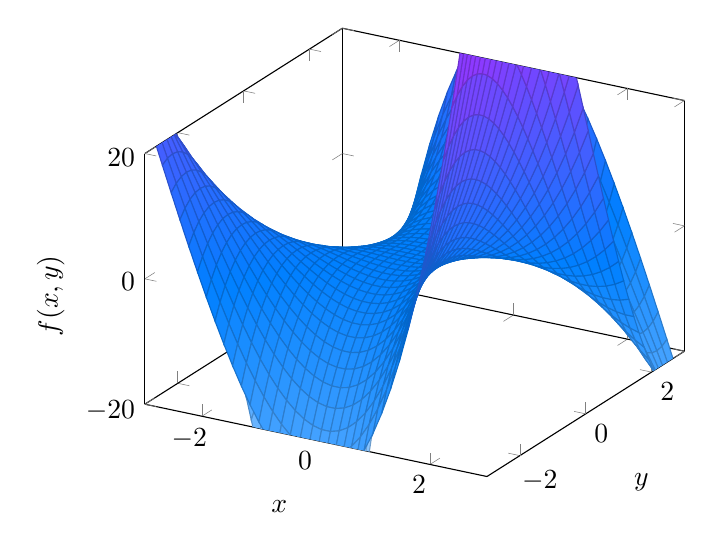
\begin{tikzpicture}
    \begin{axis}[
        view={30}{30},        % Angle de vue
        colormap/cool,        % Colormap pour les couleurs
        domain=-3:3,          % Domaine des variables x et y
        samples=40,           % Nombre d'échantillons
        xlabel=$x$,           % Étiquette pour l'axe x
        ylabel=$y$,           % Étiquette pour l'axe y
        zlabel={$f(x,y)$},    % Étiquette pour l'axe z
        zmax=20,              % Limite maximale de l'axe z
        zmin=-20              % Limite minimale de l'axe z
    ]
    \addplot3[
        surf,                 % Style de tracé en surface
    ]
    {x^3 - 3*x^2*y + y^3};    % Fonction à tracer
    \end{axis}
\end{tikzpicture} }
\end{enumerate} } 
}